%! Licence = CC BY-NC-SA 4.0

%! Author = gianfluetsch
%! Date = 30. Dez 2021
%! Project = cydef_summary

\section{MISP}
MISP Threat Sharing (MISP) is an open source threat intelligence platform. The project develops utilities and documentation for more effective threat intelligence, by sharing indicators of compromise.\\

OSINT: GitHub, MalwareBazaar, URLhaus, Tweetdeck\\
CSINT: Mail, PDF\\
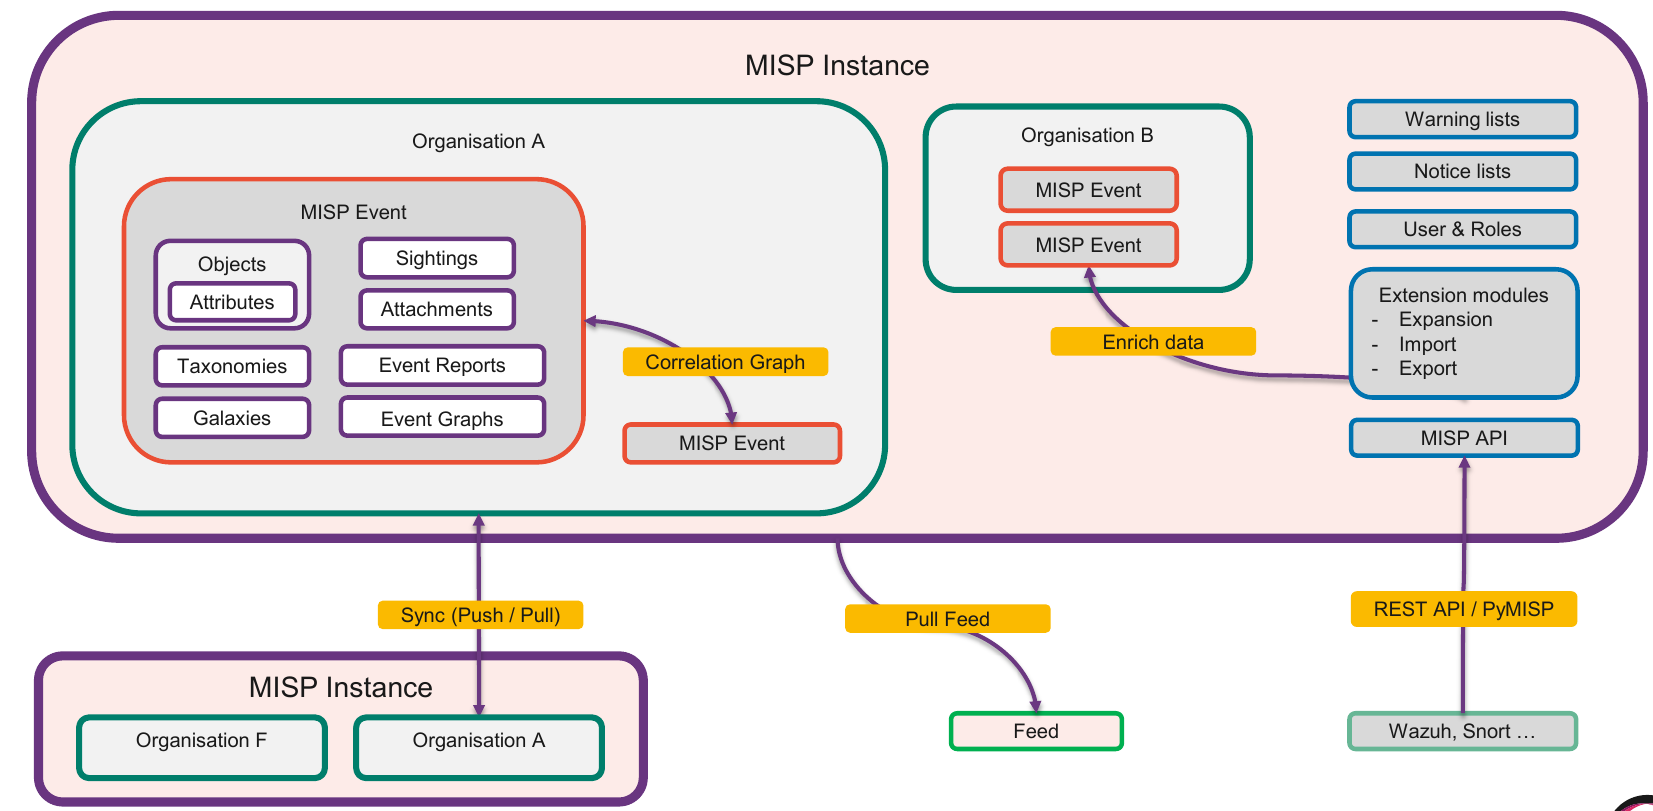
\includegraphics[width=\linewidth]{./img/15-misp/misp.png}
\begin{itemize}
    \item MISP software facilitates the exchange and sharing of:
    \begin{itemize}
        \item threat intelligence
        \item Indicators of Compromise (IoCs)
        \item Targeted malware and attacks
        \item financial fraud
        \item or any intelligence within your community of trusted members.
    \end{itemize}
    \item Used by malware researchers and SOC's
    \item More than 6000 organisations worldwide are using MISP
\end{itemize}

\subsection{Events}
\begin{itemize}
    \item MISP events are encapsulations for contextually related information represented as attribute and object.
    \item Used to store and share malware data / IOCs in a structured way
    \item Foundation of MISP
    \item Can be shared to other MISP instances
    \item Always belongs to one organisation
\end{itemize}
Events include: Date, Distribution, Threat Level, Analysis, Event Info, Extends Event

\subsection{Attributes}
\begin{itemize}
    \item Describe a MISP event
    \item can be network indicators (e.g. IP address)
    \item can be system indicators (e.g. a string in memory)
    \item can be even bank account details
    \item can be Many more ...
\end{itemize}

\subsection{Categories and Types}
Categories:
\begin{itemize}
    \item Financial fraud
    \item Network activity
    \item Payload installation
    \item Person
\end{itemize}
Types:
\begin{itemize}
    \item Btc (bitcoin address)
    \item Email-body
    \item Ip-src  
\end{itemize}

\subsection{Objects}
Groups attributes which belong together.\\
Person object $\rightarrow$ Attributes: Last Name, First Name, Portrait, Address, Phone Number, birth date\\
Email object $\rightarrow$ Attributes: Screenshot, Reply-to, Subject, To, From, Msg, From-domain
\subsection{Attachments}
File attachments can be added to Categories
\begin{itemize}
    \item Antivirus detection
    \item Payload delivery
    \item Artifacts dropped
    \item Payload installation
    \item Network activity (e.g. Wireshark PCAP file)
    \item External analysis (e.g. Report from online sandbox)
    \item Support Tool (e.g. Support Ticket PDF)
\end{itemize}
Is a malware sample (encrypt and hash) $\rightarrow$ Creates file object (file, filename, md5, sha1, sha256, size)\\
Advanced extraction $\rightarrow$ Creates additional attributes (entropy, mimetype, ssdeep, ...)

\subsection{Import}
Import can be Freetext or Template.

\subsection{Graphs}
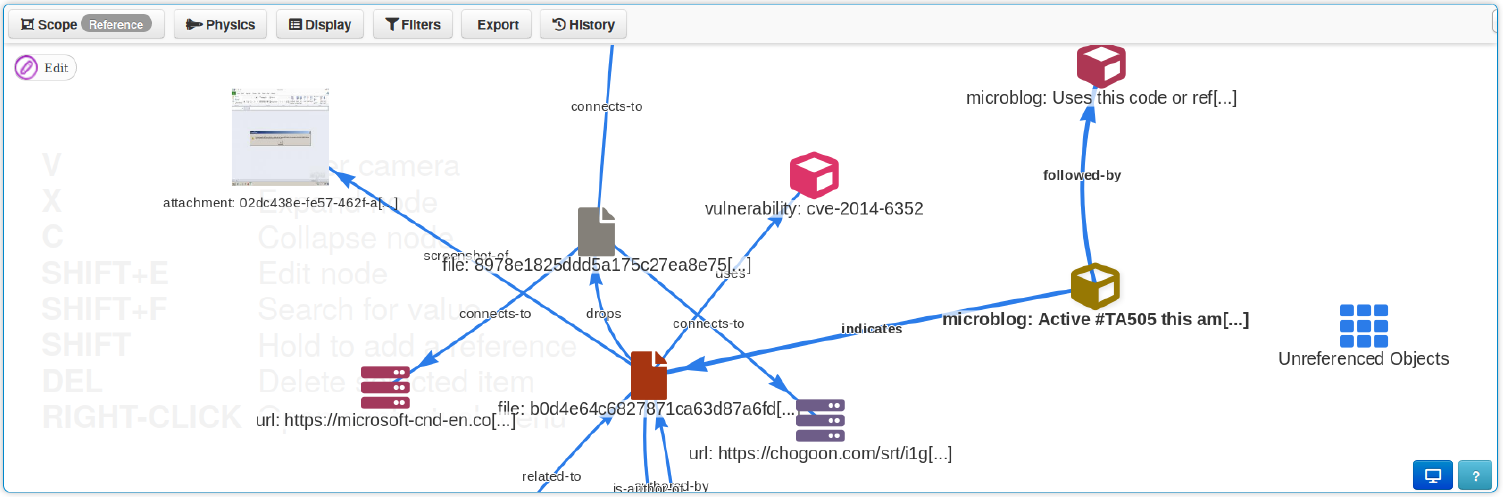
\includegraphics[width=\linewidth]{./img/15-misp/graph}

\subsection{Taxonomies}
\begin{itemize}
    \item Classify your events
    \item Admin must enable them separately
    \item A Taxonomy Library contains several tags
    \item Tags can be set on attributes or events\\
\end{itemize}
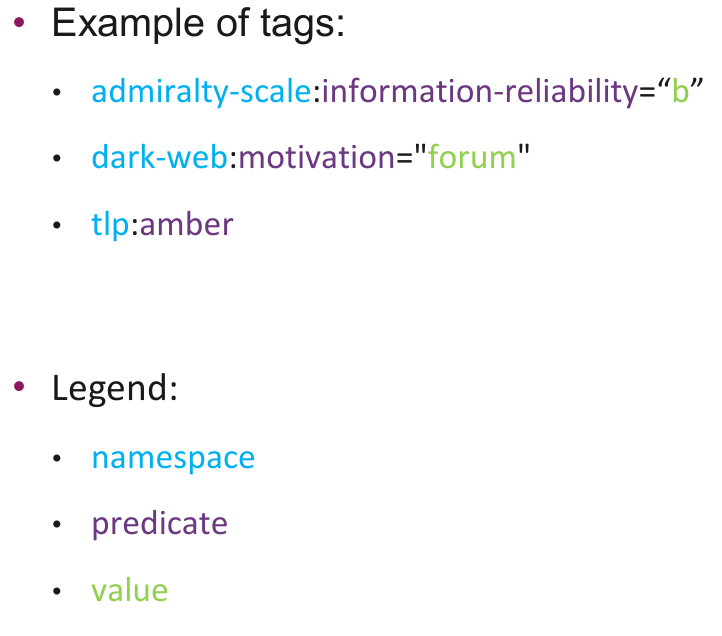
\includegraphics[width=.7\linewidth]{./img/15-misp/misp_tag}\\
\textbf{Use cases:}
\begin{itemize}
    \item Display all events with a specific tag
    \item Classification for sharing
    \item Filtering mechanisms to rename or replacetaxonomies/tags at pull and push synchronisation
    \item Set events for further processing by external tools
\end{itemize}

\columnbreak

\subsection{Galaxies}
Galaxies in MISP are a method used to express a large object called cluster.
Can be attached to MISP events or attributes
A cluster can be composed of one or more elements.
Elements are expressed as key-values.
\subsection{Sightings}
provide method to signal false positives\\
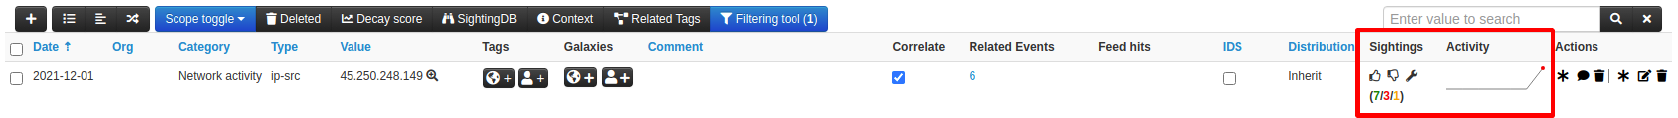
\includegraphics[width=\linewidth]{./img/15-misp/sightings.png}
\subsection{Event Report}
Event report can be generated on an event. compiled to markdown from the already given attributes / objects or hand written.\\
\textbf{Proposals} can be generated. Owner of event can approve or discard the proposal
\subsection{Correlation}
MISP automatically creates correlations. Relationship between events: Matching file hash, Matching email address, Matching IP address
\subsection{Warning Lists}
MISP warninglists are lists of well-known indicators that can be associated to potential false positives, errors or mistakes.
\subsection{Notice Lists}
Inform MISP users of Legal implications, Privacy implications, Policy implications, Technical implications.
Currently only gdpr.
\subsection{Sharing}
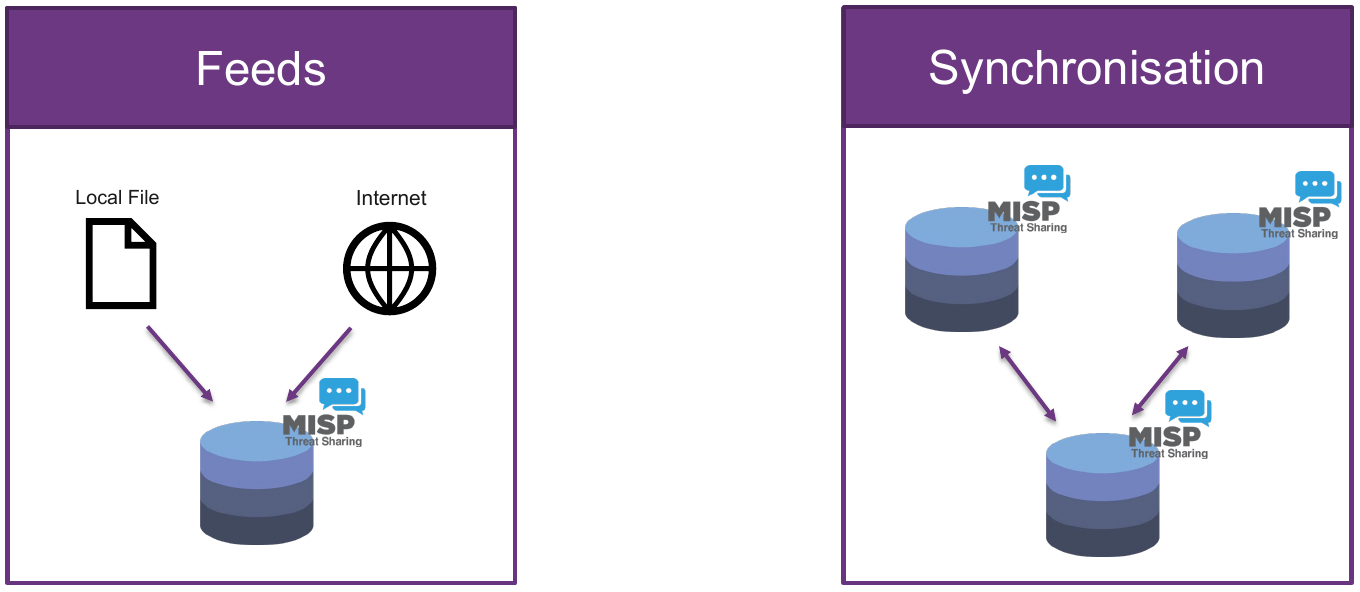
\includegraphics[width=\linewidth]{./img/15-misp/sharing.png}
\subsubsection{Distribution Levels}
Events that are not published are only distributed to the local organisations on the same MISP server
\begin{itemize}
    \item Your organisation only
    \item This community only
    \item Connected communities
    \item All communities
    \item Sharing group
\end{itemize}
Only events that are published will be shared with other MISP servers via push / pull mechanisms
\subsubsection{Feeds}
Easily import any remote or local URL to store the data in your MISP instance at regular intervals.
\subsubsection{Synchronisation}
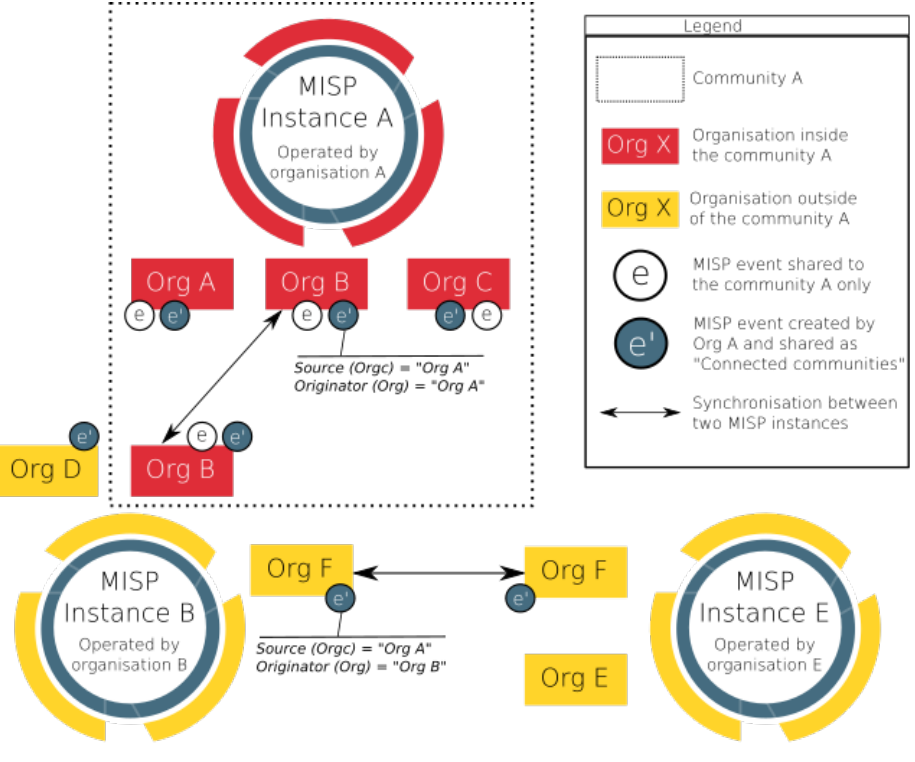
\includegraphics[width=\linewidth]{./img/15-misp/misp_synchronisation.png}
A MISP Server you want to sync with is a \textbf{Sync Server}. API credentials of sync user are needed.
\begin{itemize}
    \item Push
    \begin{itemize}
        \item Provides a seemingly real time experience
        \item Attempt to synchronise is made immediately after publication of an event
        \item Disadvantage: connection issues or dead workers might prevent the push from being successful
        \item Data with distribution set to Your organisation only or This community only will not be synchronised
    \end{itemize}
    \item Pull
    \begin{itemize}
        \item Only performed on command
        \item Could be a manual trigger by an admin or a cron job
        \item Will also fetch objects with a distribution set to this community only and organisation only
       
    \end{itemize}
\end{itemize}
\subsection{Sharing Groups}
More granular way to create re-usable distribution lists for events/attributes. Can be created by User. Not recommended in practice.

\subsection{API}
MISP REST API allows for third parties to access MISP database. API AuthKey is needed. Access via REST or PyMISP.
\subsection{Expansion Modules}
Extend functionality beyond MISP’s core features. 

\begin{itemize}
    \item Expansion modules (BTC scam check, GeoIP, JoeSandbox Submit, ...)
    \item Export modules (PDF Export, Cisco ACL rule, ...)
    \item Import modules (CSV Import, Email import, OCR ...)
\end{itemize}

\subsection{Introduction}

\subsubsection{MISP Usage}
MISP is used for collecting and categorizing malware samples. These events can then be shared und used for other communities.

\subsubsection{Feed}
The feeds can be used as a source of correlations for all of your events and attributes without the need to import them directly into your system. The MISP feed system allows for fast correlation but also a for quick comparisons of the feeds against one another.

\subsection{Phishing Email}

\subsubsection{Difference Attributes \& Objects in an event}
An attribute is a single value stored in MISP with a specific category. An object in opposite, is like a collection of attributes, which are related together (for example: Person - first name and last name are together an object, if they are not linked, then they are attributes)

\subsubsection{Why are you just able to merge to person object and not to a employee object?}
There aren't enough parameter provided for MISP in order to merge to an employee object.

\subsubsection{Why does the IP address not show up as a correlation between the two events?}
The sender email address is the same, but google sent the mail from different mailserver, so the ip address is different. That means, that MISP isn't able to correlate them by the IP address.

\subsection{Malware Sandbox}

\subsubsection{Describe the advantages \& disadvantages of uploading the file directly to MISP vs. uploading the file to a sandbox}
Malware samples are dangerous. Therefore we can use Sandboxes to see what effect certain malicious files have on a certain system and if they do any harm. Advantages to uploading the Malware to a online sandbox (like Hybrid-Analysis) are that they gather information about the file(s) from different sources (virus total etc.) and they are accessible from a browser. This makes it very convenient to test malicious files.
On the other hand, a file can be uploaded directly to MISP. The instance then created a set of hashes of that file which can lead to correlation of other events later. This makes it useful to identify if the file already has appeared elsewhere.
In the end, a combination of using a online malware sandbox and MIPS's internal tools is the best option.

\subsubsection{Please examine the following correlation graph. Describe what you can interpret from the given data}
\begin{center}
    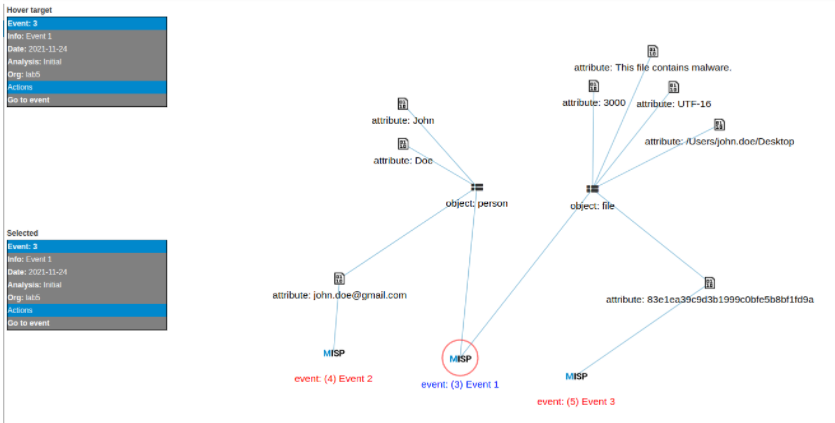
\includegraphics[width=1.0\linewidth]{misp_sandbox}
    \vspace{-8pt}
\end{center}

The graph shows three events that correlate in some way with each other. We are currently looking from Event 1's point of view. Event 2 has a connection to the attribute john.doe@gmail.com which connects to Event 1. Event 1 then has connection to Event 3 over a file hash.
The graph also shows other attributes of the file object and person object, like first name, last name, file size, file path and so on.
The graph gives a quick overview of how the attributes correlate. To go further in detail, the events can be viewed individually.

\subsection{API}

\subsubsection{Describe what you can do with the MISP API and who might use this API}
MISP can and will be used in combination with other tools. For example a firewall might needs access to certain parts of information that MISP collects. This could be a feed of bad IPs, that MISP collects and the firewall then enforces rules to prevent access to those IPs.

\subsubsection{Python Script}
PThe following script will return if the event is published, how many attributes the event has and what distribution level it has.

\begin{lstlisting}[language=Python]
    from pymisp import PyMISP

    misp_url = "http://localhost:10000/"
    misp_key = "eFCeKeKFq6BJIVzHrzTUxW7pYoN0hj0Xur9ca0vV"
    misp_verifycert = False

    myMispInstance = PyMISP(misp_url, misp_key, misp_verifycert)
    event = myMispInstance.get_event(6)

    print(f"Event published: {event['Event']['published']}")
    print(f"Attribute Count: {event['Event']['attribute_count']}")
    print(f"Distribution Level: {event['Event']['distribution']}")
\end{lstlisting}



\subsection{Event Graph | MITRE ATT\&CK}

\subsubsection{What are advantages of using the MISP event graph?}
Nobody likes reading through long paragraphs of documentation. Get a little summary by the graphics, how the objects and/or attributes are linked is more userfriedly. And the researcher will save time too!

\subsubsection{What is the difference between tags and galaxies in MISP?}
MISP galaxies are a method used to express a large object (called cluster) that can be attached to MISP events or attributes (way to attach more complex structures to data). There are default vocabularies available in MISP galaxy from existing standards (like STIX, Veris, ATT\&CK, ...) or your MISP site administrator can create custom ones for you.\\

Tag are uses to tag events, objects or attributes (obviously). Tags can be set from Taxonomy or Custom tags. Example for an tag could be "tlp:white"

\subsection{Sharing}

\subsubsection{On your instance A, you defined the distribution level of this event as Community only, but on instance B the distribution level is set to Organisation - Why?}
The distribution level can vary from instance to instance. The highest level is always at the organisation which created (and owns) the event.

\subsubsection{Why is it NOT necessary to update the distribution level of this event?}
Org F (on the same instance) cannot see the event.

\subsubsection{To which other MISP instances will the MISP instance B forward the Hello World from Org A event?}
The event will be shared to all instances, because the distribution level is set to All communities.

\subsubsection{Difference between the synchronisation philosophy and feeds in MISP?}
Feeds lets you pull data from an URL (external sources) or files. On the other hand synchronisation lets you pull or / and push event between multiple MISP instances.

\subsection{Expansion Modules}

\subsubsection{Why should even foreign (trustworthy) Modules be used?}
They could support you during research. MISP Modules can save you a lot of repetitive work

\subsubsection{Why does MISP introduced a feature like Modules, when it's already open source?}
No one is able to develop a tool that satisfies all users with all their desired features. So MISP invented Modules wich can be used like mods in games.



\subsection{Warning Lists}

\subsubsection{Explain why this information (warning lists) is useful and how investigators might use this feature.}
This information can be very valuable for someone who adds an event. The information that a certain IP address belongs to for example a Google IP range can be a useful hint. The ability to enable and disable the warninglists individually can be useful as well, because not every list is relevant for every organisation.

\subsubsection{Why does the value bit.ly set off two warning?}
This value appears in two lists. It is in the URL Shorteners domain and Office 365 URLs list included.

\subsubsection{Try to add a second attribute to the event and add a value also in one of the enabled warninglists. Does it also show up as a warning?}
As long as the value added is in the correct category and type (and in the warninglist) the attribute warning shows up like this.

